\documentclass[12pt, a4paper, oneside]{ctexart}
\usepackage{amsmath, amsthm, amssymb, bm, color, graphicx, geometry, mathrsfs,extarrows, braket, booktabs, array, wrapfig, enumitem}
\usepackage[colorlinks,linkcolor=red,anchorcolor=blue,citecolor=blue,urlcolor=blue,menucolor=black]{hyperref}
%%%% 设置中文字体 %%%%
% fc-list -f "%{family}\n" :lang=zh >d:zhfont.txt 命令查看已有字体
\setCJKmainfont{方正书宋.ttf}[BoldFont = 方正黑体_GBK.ttf, ItalicFont = simkai.ttf, BoldItalicFont = 方正粗楷简体.ttf]
%%%% 设置英文字体 %%%%
\setmainfont{Times New Roman}
\setsansfont{Calibri}
\setmonofont{Consolas}

%%%% 设置代码块 %%%%
% 在vscode中使用minted需要先配置python解释器, Ctrl+Shift+P, 输入Python: Select Interpreter选择安装了Pygments的Python版本. 再在setting.json中xelatex和pdflatex的参数中加入 "--shell-escape", 即可
% TeXworks中配置方法参考: https://blog.csdn.net/RobertChenGuangzhi/article/details/108140093
\usepackage{minted}
\renewcommand{\theFancyVerbLine}{
    \sffamily\textcolor[rgb]{0.5,0.5,0.5}{\scriptsize\arabic{FancyVerbLine}}} % 修改代码前序号大小
% 加入不同语言的代码块
\newmintinline{cpp}{fontsize=\small, linenos, breaklines, frame=lines}
\newminted{cpp}{fontsize=\small, baselinestretch=1, linenos, breaklines, frame=lines}
\newmintedfile{cpp}{fontsize=\small, baselinestretch=1, linenos, breaklines, frame=lines}
\newmintinline{matlab}{fontsize=\small, linenos, breaklines, frame=lines}
\newminted{matlab}{fontsize=\small, baselinestretch=1, mathescape, linenos, breaklines, frame=lines}
\newmintedfile{matlab}{fontsize=\small, baselinestretch=1, linenos, breaklines, frame=lines}
\newmintinline{python}{fontsize=\small, linenos, breaklines, frame=lines, python3}  % 使用\pythoninline{代码}
\newminted{python}{fontsize=\small, baselinestretch=1, linenos, breaklines, frame=lines, python3}  % 使用\begin{pythoncode}代码\end{pythoncode}
\newmintedfile{python}{fontsize=\small, baselinestretch=1, linenos, breaklines, frame=lines, python3}  % 使用\pythonfile{代码地址}

%%%% 设置行间距与页边距 %%%%
\linespread{1.4}
%\geometry{left=2.54cm,right=2.54cm,top=3.18cm,bottom=3.18cm}
\geometry{left=1.84cm,right=1.84cm,top=2.18cm,bottom=2.18cm}

%%%% 图片相对路径 %%%%
\graphicspath{{figures/}} % 当前目录下的figures文件夹, {../figures/}则是父目录的figures文件夹
\setlength{\abovecaptionskip}{-0.2cm}  % 缩紧图片标题与图片之间的距离
\setlength{\belowcaptionskip}{0pt} 

%%%% 缩小item,enumerate,description两行间间距 %%%%
\setenumerate[1]{itemsep=0pt,partopsep=0pt,parsep=\parskip,topsep=5pt}
\setitemize[1]{itemsep=0pt,partopsep=0pt,parsep=\parskip,topsep=5pt}
\setdescription{itemsep=0pt,partopsep=0pt,parsep=\parskip,topsep=5pt}

%%%% 自定义公式 %%%%
\everymath{\displaystyle} % 默认全部行间公式
\DeclareMathOperator*\uplim{\overline{lim}} % 定义上极限 \uplim_{}
\DeclareMathOperator*\lowlim{\underline{lim}} % 定义下极限 \lowlim_{}
\DeclareMathOperator*{\argmax}{arg\,max}  % 定义取最大值的参数 \argmax_{}
\DeclareMathOperator*{\argmin}{arg\,min}  % 定义取最小值的参数 \argmin_{}
\let\leq=\leqslant % 将全部leq变为leqslant
\let\geq=\geqslant % geq同理
\DeclareRobustCommand{\rchi}{{\mathpalette\irchi\relax}}
\newcommand{\irchi}[2]{\raisebox{\depth}{$#1\chi$}} % 使用\rchi将\chi居中

%%%% 自定义环境配置 %%%%
\newcounter{problem}  % 问题序号计数器
\newenvironment{problem}[1][]{\stepcounter{problem}\par\noindent\textbf{题目\arabic{problem}. #1}}{\smallskip\par}
\newenvironment{solution}[1][]{\par\noindent\textbf{#1解答. }}{\smallskip\par}  % 可带一个参数表示题号\begin{solution}{题号}
\newenvironment{note}{\par\noindent\textbf{注记. }}{\smallskip\par}
\newenvironment{remark}{\begin{enumerate}[label=\textbf{注\arabic*.}]}{\end{enumerate}}
\BeforeBeginEnvironment{minted}{\vspace{-0.5cm}}  % 缩小minted环境距上文间距
\AfterEndEnvironment{minted}{\vspace{-0.2cm}}  % 缩小minted环境距下文间距

%%%% 一些宏定义 %%%%
\def\bd{\boldsymbol}        % 加粗(向量) boldsymbol
\def\disp{\displaystyle}    % 使用行间公式 displaystyle(默认)
\def\weekto{\rightharpoonup}% 右半箭头
\def\tsty{\textstyle}       % 使用行内公式 textstyle
\def\sign{\text{sign}}      % sign function
\def\wtd{\widetilde}        % 宽波浪线 widetilde
\def\R{\mathbb{R}}          % Real number
\def\N{\mathbb{N}}          % Natural number
\def\Z{\mathbb{Z}}          % Integer number
\def\Q{\mathbb{Q}}          % Rational number
\def\C{\mathbb{C}}          % Complex number
\def\K{\mathbb{K}}          % Number Field
\def\P{\mathbb{P}}          % Polynomial
\def\d{\mathrm{d}}          % differential operator
\def\e{\mathrm{e}}          % Euler's number
\def\i{\mathrm{i}}          % imaginary number
\def\re{\mathrm{Re}}        % Real part
\def\im{\mathrm{Im}}        % Imaginary part
\def\res{\mathrm{Res}}      % Residue
\def\ker{\mathrm{Ker}}      % Kernel
\def\vspan{\mathrm{vspan}}  % Span  \span与latex内核代码冲突改为\vspan
\def\L{\mathcal{L}}         % Loss function
\def\O{\mathcal{O}}         % big O notation
\def\wdh{\widehat}          % 宽帽子 widehat
\def\ol{\overline}          % 上横线 overline
\def\ul{\underline}         % 下横线 underline
\def\add{\vspace{1ex}}      % 增加行间距
\def\del{\vspace{-1.5ex}}   % 减少行间距

%%%% 定理类环境的定义 %%%%
\newtheorem{theorem}{定理}

%%%% 基本信息 %%%%
\newcommand{\RQ}{\today} % 日期
\newcommand{\km}{强化学习} % 科目
\newcommand{\bj}{强基数学002} % 班级
\newcommand{\xm}{吴天阳} % 姓名
\newcommand{\xh}{2204210460} % 学号

\begin{document}

%\pagestyle{empty}
\pagestyle{plain}
\vspace*{-15ex}
\centerline{\begin{tabular}{*5{c}}
    \parbox[t]{0.25\linewidth}{\begin{center}\textbf{日期}\\ \large \textcolor{blue}{\RQ}\end{center}} 
    & \parbox[t]{0.2\linewidth}{\begin{center}\textbf{科目}\\ \large \textcolor{blue}{\km}\end{center}}
    & \parbox[t]{0.2\linewidth}{\begin{center}\textbf{班级}\\ \large \textcolor{blue}{\bj}\end{center}}
    & \parbox[t]{0.1\linewidth}{\begin{center}\textbf{姓名}\\ \large \textcolor{blue}{\xm}\end{center}}
    & \parbox[t]{0.15\linewidth}{\begin{center}\textbf{学号}\\ \large \textcolor{blue}{\xh}\end{center}} \\ \hline
\end{tabular}}
\begin{center}
    \zihao{3}\textbf{第二章作业}
\end{center}\vspace{-0.2cm}
\begin{problem}[练习2.2]
    考虑一个$k=4$的多臂赌博机问题,记做$1,2,3,4$. 使用$\varepsilon$-贪心动作选择,基于均值的动作价值估计,
    初始估计$Q_1(a) = 0,\forall a=\{1,2,3,4\}$,假设动作及收益的序列为
    \begin{align*}
        A = \{1,2,2,2,3\},\ R = \{-1, 1, -2, 2, 0\}
    \end{align*}
    其中某些时刻中,可能发生了进行了探索($\varepsilon$-时刻),即随机选择一个动作.
    请问上述时间序列中,有哪些时刻肯定进行了探索?那些时刻可能进行了探索?
\end{problem}
\begin{solution}
上述序列对应的每个时刻的动作价值$Q_t(a)$变换如下表所示,从该表容易得出,第$4,5$步的选择一定是进行了探索,而所有时刻都可能进行探索,
因为在探索中,每个动作被选择到的概率是相同的.
\renewcommand\arraystretch{0.8} % 设置表格高度为原来的0.8倍
\begin{table}[!htbp] % table标准
    \centering % 表格居中
    \begin{tabular}{p{1cm}<{\centering}p{1cm}<{\centering}p{1cm}<
        {\centering}p{1cm}<{\centering}p{1cm}<{\centering}p{1cm}<
        {\centering}p{1cm}<{\centering}} % 设置表格宽度
    %\begin{tabular}{cccc}
        \toprule
$t$      & 1 & 2  & 3  & 4    & 5   & 6   \\
        \midrule
$Q_t(1)$ & 0 & -1 & -1 & -1   & -1  & -1  \\
$Q_t(2)$ & 0 & 0  & 1  & -0.5 & 1/3 & 1/3 \\
$Q_t(3)$ & 0 & 0  & 0  & 0    & 0   & 0   \\
$Q_t(4)$ & 0 & 0  & 0  & 0    & 0   & 0   \\
$A_t$    & 1 & 2  & 2  & 2    & 3   &    \\
        \bottomrule
    \end{tabular}
\end{table}
\end{solution}
\vspace*{-0.3cm}
\begin{figure}[htbp]
    \centering
    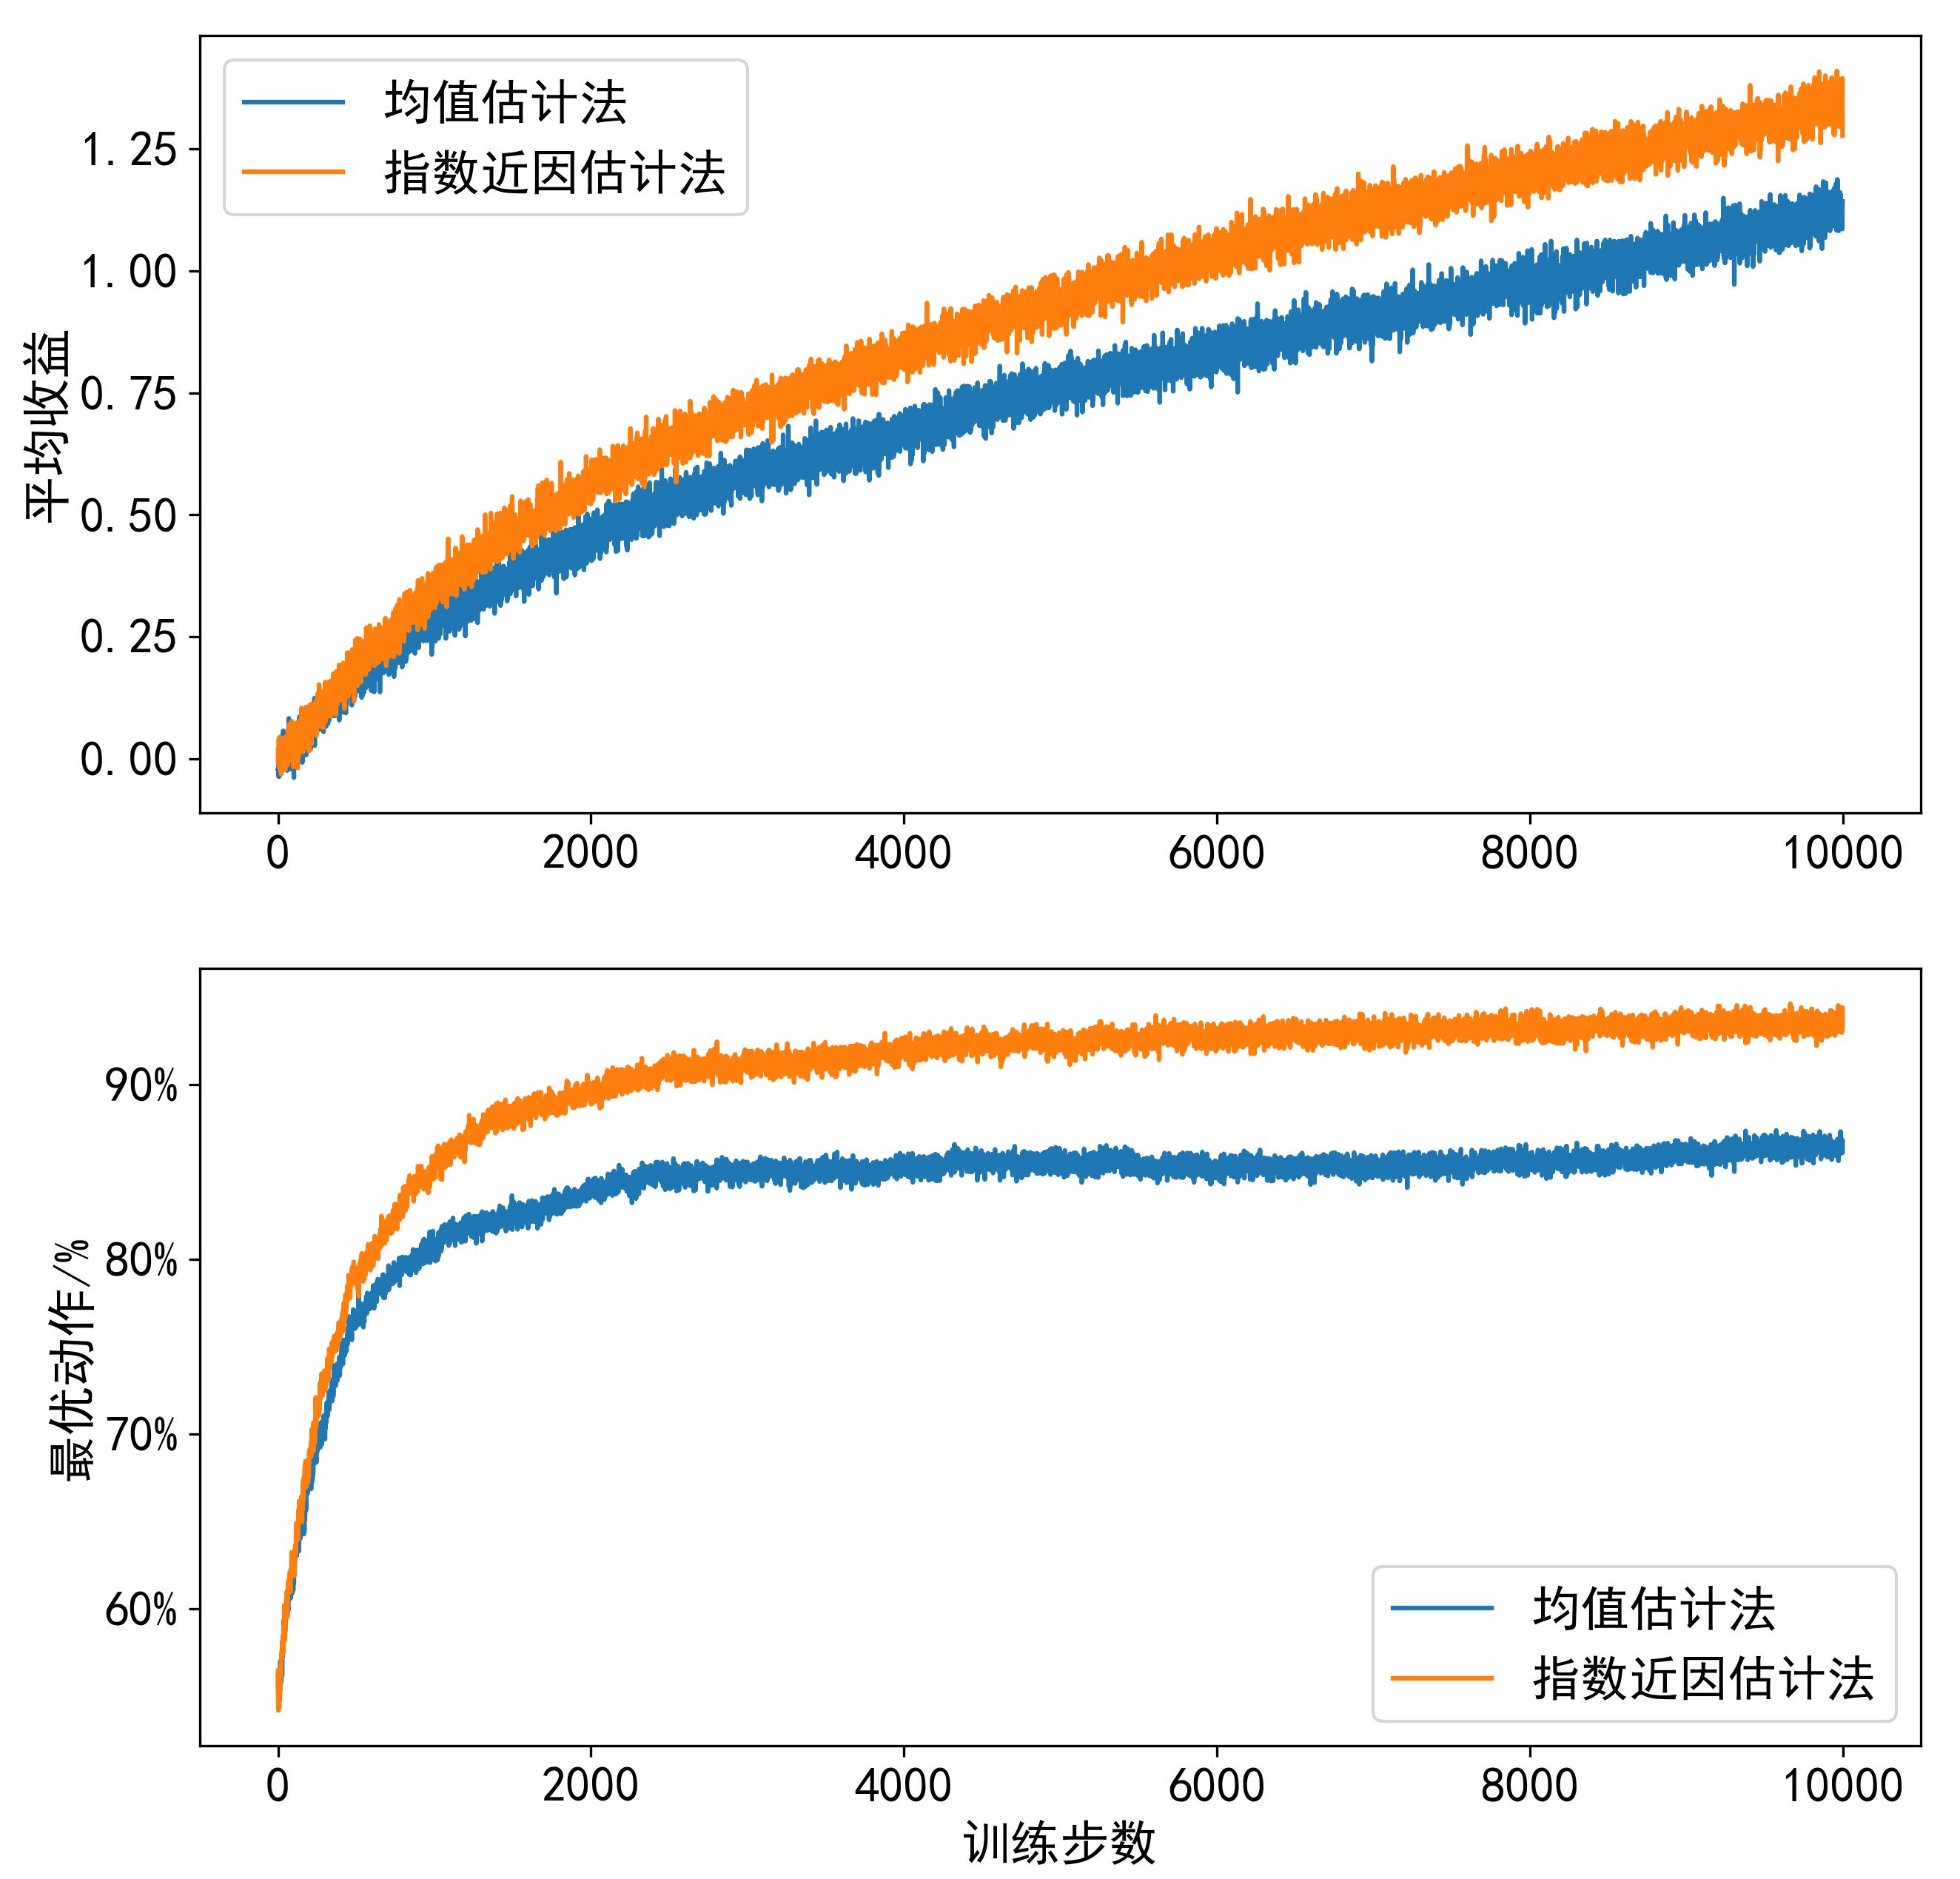
\includegraphics[scale=0.13]{033页练习2.5.png}
\end{figure}
\begin{problem}[练习2.5]
    设计实验来证实使用均值估计方法取解决非平稳问题的困难,使用一个10臂赌博机,其中所有的$q_*(a)$初始时均相等,
    然后进行随机游走,每一步所有的$q_*(a)$都加上一个服从$N(0,0.01^2)$的增量,分别使用均值估计方法和
    指数近因加权估计方法且步长$\alpha=0.1$进行决策,采用$\varepsilon$-贪心进行动作选择,且总步数为$T=10000$.
\end{problem}
\begin{solution}
    如上图所示进行了2000次不同的多臂赌博机实验的平均结果,从中非常容易得出,指数近因估计在处理多臂赌博机问题上
    比均值估计要好.
    \begin{pythoncode}
from tqdm import tqdm
import numpy as np
import matplotlib as mpl
import matplotlib.pyplot as plt

config = {  # matplotlib绘图配置
    "figure.figsize": (6, 6),  # 图像大小
    "font.size": 16, # 字号大小
    "font.sans-serif": ['SimHei'],   # 用黑体显示中文
    'axes.unicode_minus': False # 显示负号
}
plt.rcParams.update(config)

class Bandit:  # 赌博机类
    def __init__(self, n, init_means=0) -> None:
        # init_means: 赌博机初始均值
        self.n = n  # 赌博机臂个数
        self.means = np.full(self.n, init_means, dtype='float')  # 均值初始值

    def move_state(self):
        return np.random.normal(0, 0.01, self.n)  # 随机游走变换函数

    def step(self, action):  # 执行一个action,并返回其收益
        assert(0 <= action < self.n)
        self.means += self.move_state()
        mean_now = self.means[action]
        rate = np.sum(self.means <= mean_now) / self.n
        return np.random.normal(self.means[action], size=1)[0], rate

def train(strategy, alpha=0.1):
    # 两种策略 average 和 recency
    bandit = Bandit(n)
    N = np.zeros(n)
    Q = np.zeros(n)
    history = [[], []]   # 存储每个时刻的收益和最优动作占比
    for t in range(T):
        if np.random.random(1)[0] < epsilon:  # 随机选取一个动作
            action = np.random.randint(0, n)
        else:  # 贪心选择最大价值的动作
            action = np.argmax(Q)
        reward, rate = bandit.step(action)
        delta = reward - Q[action]
        N[action] += 1
        Q[action] +=  delta / N[action] if strategy == 'average' else delta * alpha
        history[0].append(reward)
        history[1].append(rate)
    return np.array(history)

def plot_reward_rate(strategy, m=2000):  # m为实验次数
    history = np.zeros((2, T))
    for _ in tqdm(range(m)):
        history += train(strategy=strategy)
    history /= m
    ax[0].plot(range(T), history[0], label='均值估计法' if strategy=='average' else '指数近因估计法')
    ax[1].plot(range(T), history[1], label='均值估计法' if strategy=='average' else '指数近因估计法')
    

if __name__ == '__main__':
    n, T = 10, 10000
    epsilon = 0.1
    np.random.seed(42)
    fig, ax = plt.subplots(2, 1, figsize=(10, 10))

    plot_reward_rate('average', m=2000)
    plot_reward_rate('recency', m=2000)

    ax[0].set_ylabel('平均收益')
    ax[1].set_ylabel('最优动作/%')
    ax[1].set_xlabel('训练步数')
    ax[1].yaxis.set_major_formatter(mpl.ticker.PercentFormatter(xmax=1, decimals=0))
    ax[0].legend()
    ax[1].legend()
    plt.savefig('33页练习2.5.png', dpi=300)
    plt.show()
    \end{pythoncode}
\end{solution}
\end{document}